\subsection{Scenario 3: Growing Infrastructure}
\add{Finish this section}
\begin{figure}[H]
    \centering
    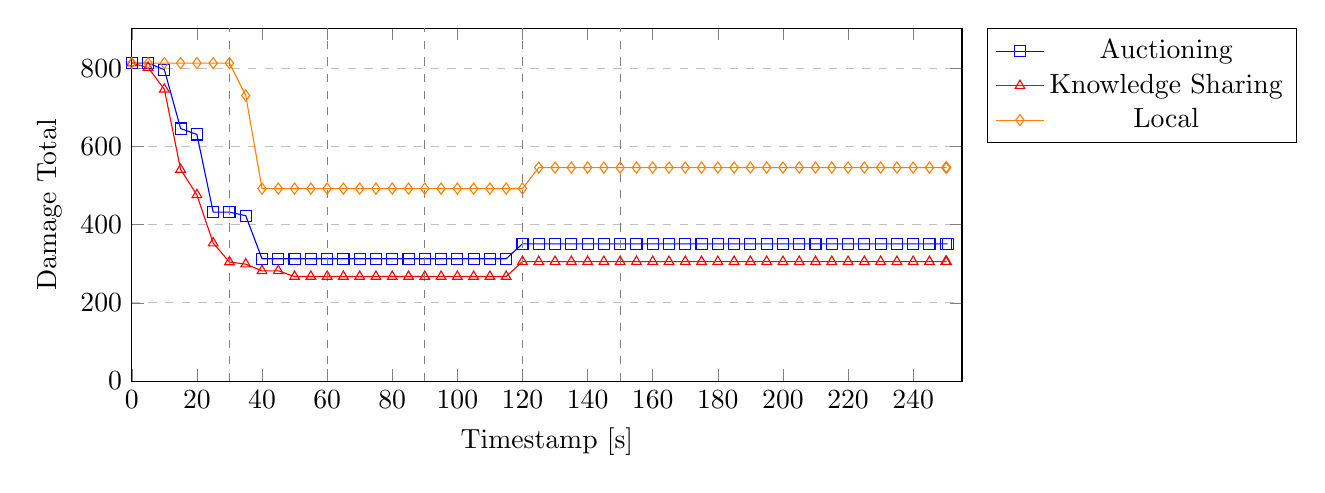
\begin{tikzpicture}
\begin{axis}[
    xlabel={Timestamp [s]},
    ylabel={Damage Total},
    xmin=0, xmax=255000,
    ymin=0, ymax=902,
    legend pos=outer north east,
    ymajorgrids=true,
    grid style=dashed,
    width=\textwidth,
    height=0.5\textwidth,
    scaled x ticks=base 10:-3,
    xtick scale label code/.code={}
]

	\addplot[color=blue,mark=square] coordinates {
        (0,812.71)(5000,812.71)(10000,796.17)(15000,645.46)(20000,630.54)(25000,431.97)(30000,431.97)(35000,422.77)(40000,312.76)(45000,312.76)(50000,312.76)(55000,312.76)(60000,312.76)(65000,312.76)(70000,312.76)(75000,312.76)(80000,312.76)(85000,312.76)(90000,312.76)(95000,312.76)(100000,312.76)(105000,312.76)(110000,312.76)(115000,312.76)(120000,350.90)(125000,350.90)(130000,350.90)(135000,350.90)(140000,350.90)(145000,350.90)(150000,350.90)(155000,350.90)(160000,350.90)(165000,350.90)(170000,350.90)(175000,350.90)(180000,350.90)(185000,350.90)(190000,350.90)(195000,350.90)(200000,350.90)(205000,350.90)(210000,350.90)(215000,350.90)(220000,350.90)(225000,350.90)(230000,350.90)(235000,350.90)(240000,350.90)(245000,350.90)(250000,350.90)(250569,350.90)
    };
    \addlegendentry{Auctioning}
	\addplot[color=red,mark=triangle] coordinates {
        (0,812.71)(5000,801.69)(10000,745.99)(15000,541.01)(20000,476.06)(25000,352.72)(30000,304.33)(35000,298.99)(40000,281.89)(45000,281.89)(50000,267.31)(55000,267.31)(60000,267.31)(65000,267.31)(70000,267.31)(75000,267.31)(80000,267.31)(85000,267.31)(90000,267.31)(95000,267.31)(100000,267.31)(105000,267.31)(110000,267.31)(115000,267.31)(120000,305.45)(125000,305.45)(130000,305.45)(135000,305.45)(140000,305.45)(145000,305.45)(150000,305.45)(155000,305.45)(160000,305.45)(165000,305.45)(170000,305.45)(175000,305.45)(180000,305.45)(185000,305.45)(190000,305.45)(195000,305.45)(200000,305.45)(205000,305.45)(210000,305.45)(215000,305.45)(220000,305.45)(225000,305.45)(230000,305.45)(235000,305.45)(240000,305.45)(245000,305.45)(250000,305.45)(250242,305.45)
    };
    \addlegendentry{Knowledge Sharing}
	\addplot[color=orange,mark=diamond] coordinates {
        (0,812.71)(5000,812.71)(10000,812.71)(15000,812.71)(20000,812.71)(25000,812.71)(30000,812.71)(35000,729.98)(40000,492.04)(45000,492.04)(50000,492.04)(55000,492.04)(60000,492.04)(65000,492.04)(70000,492.04)(75000,492.04)(80000,492.04)(85000,492.04)(90000,492.04)(95000,492.04)(100000,492.04)(105000,492.04)(110000,492.04)(115000,492.04)(120000,492.04)(125000,545.78)(130000,545.78)(135000,545.78)(140000,545.78)(145000,545.78)(150000,545.78)(155000,545.78)(160000,545.78)(165000,545.78)(170000,545.78)(175000,545.78)(180000,545.78)(185000,545.78)(190000,545.78)(195000,545.78)(200000,545.78)(205000,545.78)(210000,545.78)(215000,545.78)(220000,545.78)(225000,545.78)(230000,545.78)(235000,545.78)(240000,545.78)(245000,545.78)(250000,545.78)(250282,545.78)
    };
    \addlegendentry{Local}

	\addplot[color=gray, dashed,] coordinates {(30000,0) (30000,902)};
	\addplot[color=gray, dashed,] coordinates {(60000,0) (60000,902)};
	\addplot[color=gray, dashed,] coordinates {(90000,0) (90000,902)};
	\addplot[color=gray, dashed,] coordinates {(120000,0) (120000,902)};
	\addplot[color=gray, dashed,] coordinates {(150000,0) (150000,902)};


\end{axis}
\end{tikzpicture}
    \caption{This graph shows the overall damage of the system in the growing scenario. The damage is shown for each of the three strategies. The vertical lines indicate the time at which a node is introduced.}
    \label{fig:overall-damage-growing}
\end{figure}


\begin{figure}[H]
    \centering
    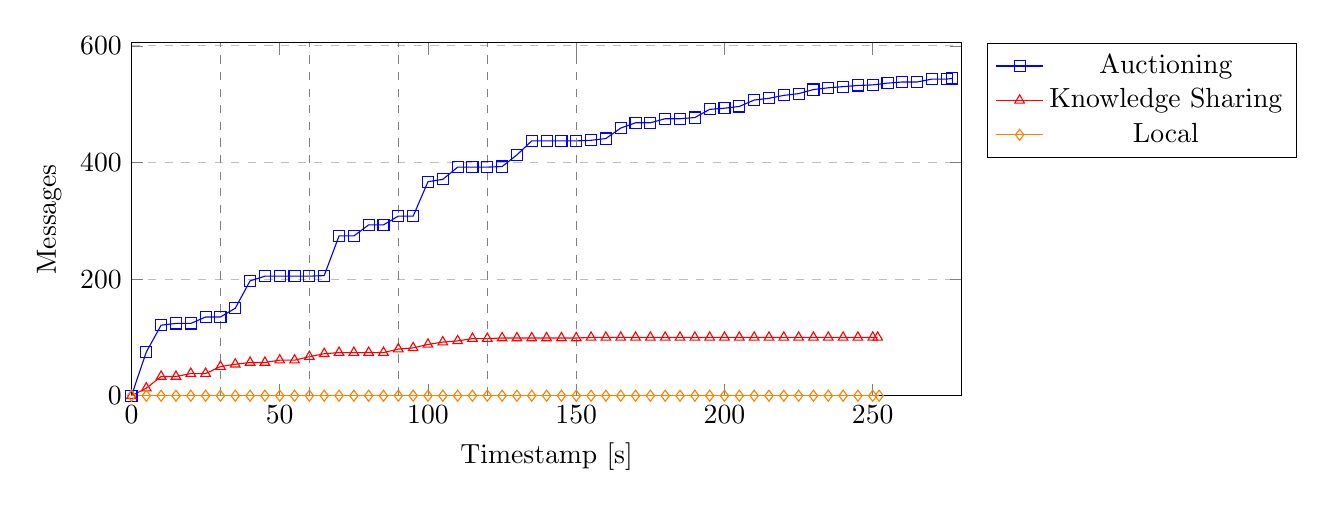
\begin{tikzpicture}
\begin{axis}[
    xlabel={Timestamp [s]},
    ylabel={Messages},
    xmin=0, xmax=280000,
    ymin=0, ymax=605,
    legend pos=outer north east,
    ymajorgrids=true,
    grid style=dashed,
    width=\textwidth,
    height=0.5\textwidth,
    scaled x ticks=base 10:-3,
    xtick scale label code/.code={}
]

	\addplot[color=blue,mark=square] coordinates {
        (0,0)(5000,75)(10000,121)(15000,124)(20000,124)(25000,135)(30000,135)(35000,150)(40000,197)(45000,205)(50000,205)(55000,205)(60000,205)(65000,206)(70000,274)(75000,274)(80000,293)(85000,293)(90000,308)(95000,308)(100000,367)(105000,371)(110000,392)(115000,392)(120000,392)(125000,393)(130000,413)(135000,437)(140000,437)(145000,437)(150000,437)(155000,438)(160000,441)(165000,459)(170000,468)(175000,468)(180000,475)(185000,475)(190000,477)(195000,491)(200000,493)(205000,496)(210000,507)(215000,510)(220000,515)(225000,518)(230000,525)(235000,528)(240000,530)(245000,532)(250000,533)(255000,536)(260000,538)(265000,538)(270000,543)(275000,543)(276704,544)
    };
    \addlegendentry{Auctioning}
	\addplot[color=red,mark=triangle] coordinates {
        (0,0)(5000,13)(10000,33)(15000,33)(20000,38)(25000,38)(30000,50)(35000,54)(40000,57)(45000,57)(50000,61)(55000,61)(60000,67)(65000,72)(70000,74)(75000,74)(80000,74)(85000,74)(90000,80)(95000,82)(100000,88)(105000,92)(110000,94)(115000,98)(120000,98)(125000,99)(130000,99)(135000,99)(140000,99)(145000,99)(150000,99)(155000,100)(160000,100)(165000,100)(170000,100)(175000,100)(180000,100)(185000,100)(190000,100)(195000,100)(200000,100)(205000,100)(210000,100)(215000,100)(220000,100)(225000,100)(230000,100)(235000,100)(240000,100)(245000,100)(250000,100)(251678,100)
    };
    \addlegendentry{Knowledge Sharing}
	\addplot[color=orange,mark=diamond] coordinates {
        (0,0)(5000,0)(10000,0)(15000,0)(20000,0)(25000,0)(30000,0)(35000,0)(40000,0)(45000,0)(50000,0)(55000,0)(60000,0)(65000,0)(70000,0)(75000,0)(80000,0)(85000,0)(90000,0)(95000,0)(100000,0)(105000,0)(110000,0)(115000,0)(120000,0)(125000,0)(130000,0)(135000,0)(140000,0)(145000,0)(150000,0)(155000,0)(160000,0)(165000,0)(170000,0)(175000,0)(180000,0)(185000,0)(190000,0)(195000,0)(200000,0)(205000,0)(210000,0)(215000,0)(220000,0)(225000,0)(230000,0)(235000,0)(240000,0)(245000,0)(250000,0)(252143,0)
    };
    \addlegendentry{Local}

	\addplot[color=gray, dashed,] coordinates {(30000,0) (30000,605)};
	\addplot[color=gray, dashed,] coordinates {(60000,0) (60000,605)};
	\addplot[color=gray, dashed,] coordinates {(90000,0) (90000,605)};
	\addplot[color=gray, dashed,] coordinates {(120000,0) (120000,605)};
	\addplot[color=gray, dashed,] coordinates {(150000,0) (150000,605)};


\end{axis}
\end{tikzpicture}
    \caption{Graph showing the total amount of messages sent between agents in the growing infrastructure scenario.}
    \label{fig:messages-growing}
\end{figure}
\begin{figure}[H]
    \centering
    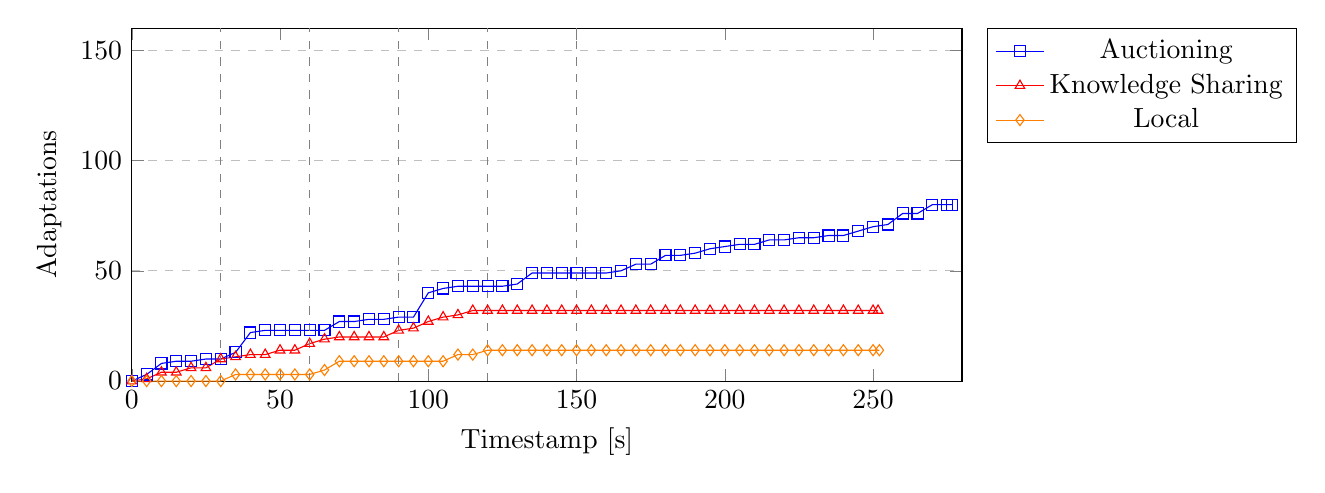
\begin{tikzpicture}
\begin{axis}[
    xlabel={Timestamp [s]},
    ylabel={Adaptations},
    xmin=0, xmax=280000,
    ymin=0, ymax=160,
    legend pos=outer north east,
    ymajorgrids=true,
    grid style=dashed,
    width=\textwidth,
    height=0.5\textwidth,
    scaled x ticks=base 10:-3,
    xtick scale label code/.code={}
]

	\addplot[color=blue,mark=square] coordinates {
        (0,0)(5000,3)(10000,8)(15000,9)(20000,9)(25000,10)(30000,10)(35000,13)(40000,22)(45000,23)(50000,23)(55000,23)(60000,23)(65000,23)(70000,27)(75000,27)(80000,28)(85000,28)(90000,29)(95000,29)(100000,40)(105000,42)(110000,43)(115000,43)(120000,43)(125000,43)(130000,44)(135000,49)(140000,49)(145000,49)(150000,49)(155000,49)(160000,49)(165000,50)(170000,53)(175000,53)(180000,57)(185000,57)(190000,58)(195000,60)(200000,61)(205000,62)(210000,62)(215000,64)(220000,64)(225000,65)(230000,65)(235000,66)(240000,66)(245000,68)(250000,70)(255000,71)(260000,76)(265000,76)(270000,80)(275000,80)(276704,80)
    };
    \addlegendentry{Auctioning}
	\addplot[color=red,mark=triangle] coordinates {
        (0,0)(5000,1)(10000,4)(15000,4)(20000,6)(25000,6)(30000,10)(35000,11)(40000,12)(45000,12)(50000,14)(55000,14)(60000,17)(65000,19)(70000,20)(75000,20)(80000,20)(85000,20)(90000,23)(95000,24)(100000,27)(105000,29)(110000,30)(115000,32)(120000,32)(125000,32)(130000,32)(135000,32)(140000,32)(145000,32)(150000,32)(155000,32)(160000,32)(165000,32)(170000,32)(175000,32)(180000,32)(185000,32)(190000,32)(195000,32)(200000,32)(205000,32)(210000,32)(215000,32)(220000,32)(225000,32)(230000,32)(235000,32)(240000,32)(245000,32)(250000,32)(251678,32)
    };
    \addlegendentry{Knowledge Sharing}
	\addplot[color=orange,mark=diamond] coordinates {
        (0,0)(5000,0)(10000,0)(15000,0)(20000,0)(25000,0)(30000,0)(35000,3)(40000,3)(45000,3)(50000,3)(55000,3)(60000,3)(65000,5)(70000,9)(75000,9)(80000,9)(85000,9)(90000,9)(95000,9)(100000,9)(105000,9)(110000,12)(115000,12)(120000,14)(125000,14)(130000,14)(135000,14)(140000,14)(145000,14)(150000,14)(155000,14)(160000,14)(165000,14)(170000,14)(175000,14)(180000,14)(185000,14)(190000,14)(195000,14)(200000,14)(205000,14)(210000,14)(215000,14)(220000,14)(225000,14)(230000,14)(235000,14)(240000,14)(245000,14)(250000,14)(252143,14)
    };
    \addlegendentry{Local}

	\addplot[color=gray, dashed,] coordinates {(30000,0) (30000,160)};
	\addplot[color=gray, dashed,] coordinates {(60000,0) (60000,160)};
	\addplot[color=gray, dashed,] coordinates {(90000,0) (90000,160)};
	\addplot[color=gray, dashed,] coordinates {(120000,0) (120000,160)};
	\addplot[color=gray, dashed,] coordinates {(150000,0) (150000,160)};


\end{axis}
\end{tikzpicture}
    \caption{Graph showing the total amount of adaptations applied by agents in the growing scenario.}
    \label{fig:proposals-growing}
\end{figure}
\begin{figure}[H]
    \centering
        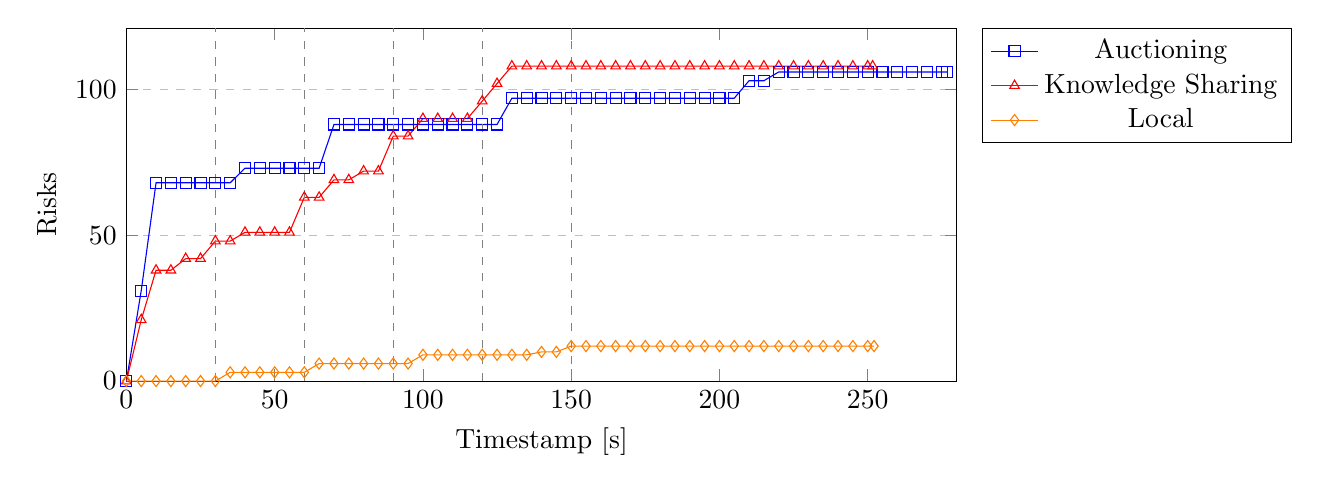
\begin{tikzpicture}
\begin{axis}[
    xlabel={Timestamp [s]},
    ylabel={Risks},
    xmin=0, xmax=280000,
    ymin=0, ymax=121,
    legend pos=outer north east,
    ymajorgrids=true,
    grid style=dashed,
    width=\textwidth,
    height=0.5\textwidth,
    scaled x ticks=base 10:-3,
    xtick scale label code/.code={}
]

	\addplot[color=blue,mark=square] coordinates {
        (0,0)(5000,31)(10000,68)(15000,68)(20000,68)(25000,68)(30000,68)(35000,68)(40000,73)(45000,73)(50000,73)(55000,73)(60000,73)(65000,73)(70000,88)(75000,88)(80000,88)(85000,88)(90000,88)(95000,88)(100000,88)(105000,88)(110000,88)(115000,88)(120000,88)(125000,88)(130000,97)(135000,97)(140000,97)(145000,97)(150000,97)(155000,97)(160000,97)(165000,97)(170000,97)(175000,97)(180000,97)(185000,97)(190000,97)(195000,97)(200000,97)(205000,97)(210000,103)(215000,103)(220000,106)(225000,106)(230000,106)(235000,106)(240000,106)(245000,106)(250000,106)(255000,106)(260000,106)(265000,106)(270000,106)(275000,106)(276704,106)
    };
    \addlegendentry{Auctioning}
	\addplot[color=red,mark=triangle] coordinates {
        (0,0)(5000,21)(10000,38)(15000,38)(20000,42)(25000,42)(30000,48)(35000,48)(40000,51)(45000,51)(50000,51)(55000,51)(60000,63)(65000,63)(70000,69)(75000,69)(80000,72)(85000,72)(90000,84)(95000,84)(100000,90)(105000,90)(110000,90)(115000,90)(120000,96)(125000,102)(130000,108)(135000,108)(140000,108)(145000,108)(150000,108)(155000,108)(160000,108)(165000,108)(170000,108)(175000,108)(180000,108)(185000,108)(190000,108)(195000,108)(200000,108)(205000,108)(210000,108)(215000,108)(220000,108)(225000,108)(230000,108)(235000,108)(240000,108)(245000,108)(250000,108)(251678,108)
    };
    \addlegendentry{Knowledge Sharing}
	\addplot[color=orange,mark=diamond] coordinates {
        (0,0)(5000,0)(10000,0)(15000,0)(20000,0)(25000,0)(30000,0)(35000,3)(40000,3)(45000,3)(50000,3)(55000,3)(60000,3)(65000,6)(70000,6)(75000,6)(80000,6)(85000,6)(90000,6)(95000,6)(100000,9)(105000,9)(110000,9)(115000,9)(120000,9)(125000,9)(130000,9)(135000,9)(140000,10)(145000,10)(150000,12)(155000,12)(160000,12)(165000,12)(170000,12)(175000,12)(180000,12)(185000,12)(190000,12)(195000,12)(200000,12)(205000,12)(210000,12)(215000,12)(220000,12)(225000,12)(230000,12)(235000,12)(240000,12)(245000,12)(250000,12)(252143,12)
    };
    \addlegendentry{Local}

	\addplot[color=gray, dashed,] coordinates {(30000,0) (30000,121)};
	\addplot[color=gray, dashed,] coordinates {(60000,0) (60000,121)};
	\addplot[color=gray, dashed,] coordinates {(90000,0) (90000,121)};
	\addplot[color=gray, dashed,] coordinates {(120000,0) (120000,121)};
	\addplot[color=gray, dashed,] coordinates {(150000,0) (150000,121)};


\end{axis}
\end{tikzpicture}
    \caption{Graph showing the number of unique risks detected by agents in the growing scenario.}
    \label{fig:risk-count-growing}
\end{figure}
\begin{figure}[H]
    \centering
        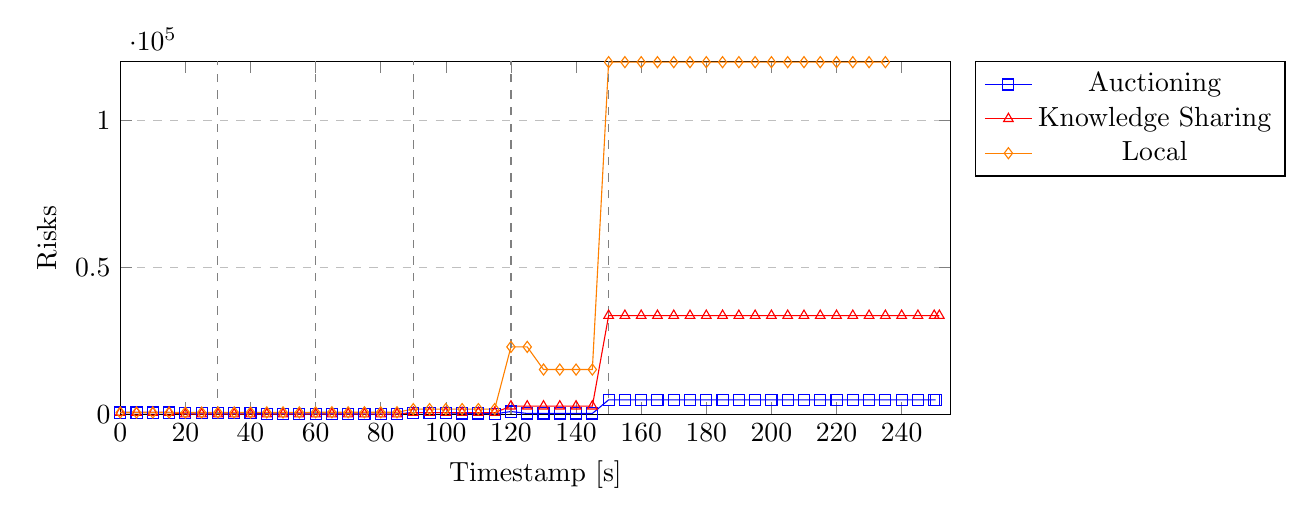
\begin{tikzpicture}
\begin{axis}[
    xlabel={Timestamp [s]},
    ylabel={Risks},
    xmin=0, xmax=255000,
    ymin=0, ymax=120012,
    legend pos=outer north east,
    ymajorgrids=true,
    grid style=dashed,
    width=\textwidth,
    height=0.5\textwidth,
    scaled x ticks=base 10:-3,
    xtick scale label code/.code={}
]

	\addplot[color=blue,mark=square] coordinates {
        (0,563)(5000,563)(10000,563)(15000,563)(20000,360)(25000,360)(30000,399)(35000,399)(40000,399)(45000,100)(50000,100)(55000,60)(60000,80)(65000,80)(70000,80)(75000,40)(80000,40)(85000,40)(90000,520)(95000,520)(100000,520)(105000,240)(110000,240)(115000,100)(120000,900)(125000,240)(130000,240)(135000,240)(140000,240)(145000,240)(150000,4880)(155000,4880)(160000,4880)(165000,4880)(170000,4880)(175000,4880)(180000,4880)(185000,4880)(190000,4880)(195000,4880)(200000,4880)(205000,4880)(210000,4880)(215000,4880)(220000,4880)(225000,4880)(230000,4880)(235000,4880)(240000,4880)(245000,4880)(250000,4880)(250452,4880)
    };
    \addlegendentry{Auctioning}
	\addplot[color=red,mark=triangle] coordinates {
        (0,563)(5000,563)(10000,563)(15000,563)(20000,10)(25000,10)(30000,40)(35000,20)(40000,20)(45000,20)(50000,20)(55000,20)(60000,40)(65000,40)(70000,40)(75000,40)(80000,40)(85000,40)(90000,520)(95000,520)(100000,520)(105000,520)(110000,520)(115000,520)(120000,2720)(125000,2720)(130000,2720)(135000,2720)(140000,2720)(145000,2720)(150000,33540)(155000,33540)(160000,33540)(165000,33540)(170000,33540)(175000,33540)(180000,33540)(185000,33540)(190000,33540)(195000,33540)(200000,33540)(205000,33540)(210000,33540)(215000,33540)(220000,33540)(225000,33540)(230000,33540)(235000,33540)(240000,33540)(245000,33540)(250000,33540)(251574,33540)
    };
    \addlegendentry{Knowledge Sharing}
	\addplot[color=orange,mark=diamond] coordinates {
        (0,563)(5000,563)(10000,563)(15000,563)(20000,563)(25000,563)(30000,608)(35000,608)(40000,608)(45000,608)(50000,608)(55000,608)(60000,653)(65000,653)(70000,653)(75000,653)(80000,653)(85000,653)(90000,1733)(95000,1733)(100000,1733)(105000,1733)(110000,1733)(115000,1733)(120000,22883)(125000,22883)(130000,15180)(135000,15180)(140000,15180)(145000,15180)(150000,119730)(155000,119730)(160000,119730)(165000,119730)(170000,119730)(175000,119730)(180000,119730)(185000,119730)(190000,119730)(195000,119730)(200000,119730)(205000,119730)(210000,119730)(215000,119730)(220000,119730)(225000,119730)(230000,119730)(235000,119730)
    };
    \addlegendentry{Local}

	\addplot[color=gray, dashed,] coordinates {(30000,0) (30000,120012)};
	\addplot[color=gray, dashed,] coordinates {(60000,0) (60000,120012)};
	\addplot[color=gray, dashed,] coordinates {(90000,0) (90000,120012)};
	\addplot[color=gray, dashed,] coordinates {(120000,0) (120000,120012)};
	\addplot[color=gray, dashed,] coordinates {(150000,0) (150000,120012)};


\end{axis}
\end{tikzpicture}
    \caption{Graph showing the number of remaining risks in the infrastructure in the growing scenario.}
    \label{fig:risk-remaining-growing}
\end{figure}

Figure \ref{fig:risk-remaining-growing} has a scale that is almost $60$ times larger than all other scenarios, and has found $212$ times more risks than initially. This can be explained by the growing size of the infrastructure, and the new edges that are introduced. A risk is defined as a path from an infrastructure node to a critical software component. As the infrastructure grows, the amount of possible paths grows exponentially. This is why the amount of risks detected is also growing exponentially. 

It should be noted that the probability and damage value of many of these risks are very low, as these critical paths can become long. This could be a reason why the overall damage (figure \ref{fig:overall-damage-growing}) is only $30$ times larger than at the start of the scenario. However, the metrics that are collected are not enough to determine the exact cause of this difference.

\begin{figure}[H]
    \centering
        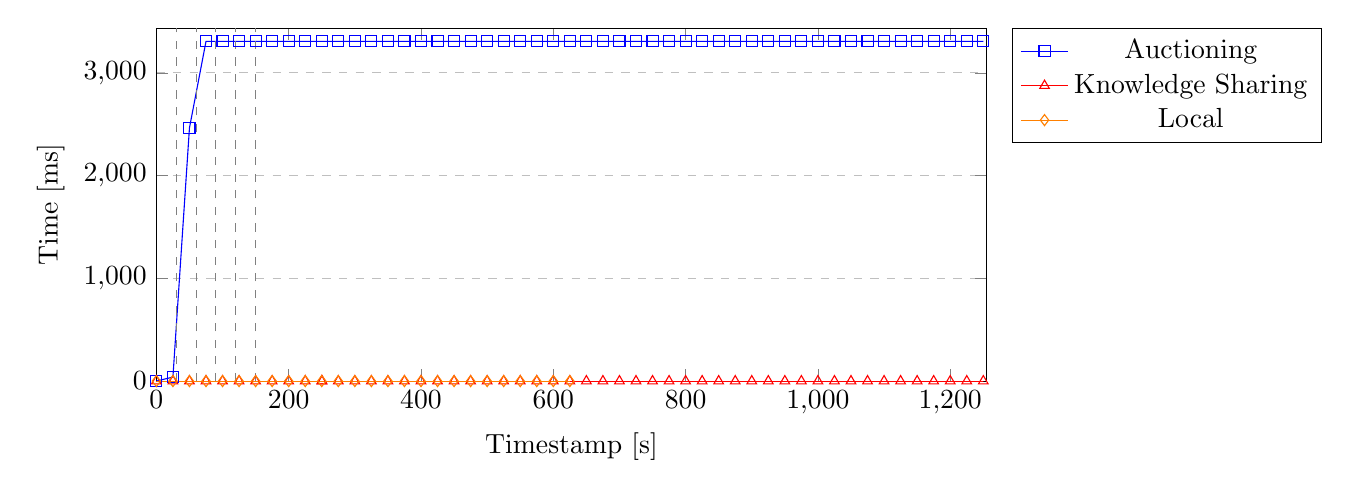
\begin{tikzpicture}
\begin{axis}[
    xlabel={Timestamp [s]},
    ylabel={Time [ms]},
    xmin=0, xmax=1255000,
    ymin=0, ymax=3434,
    legend pos=outer north east,
    ymajorgrids=true,
    grid style=dashed,
    width=\textwidth,
    height=0.5\textwidth,
    scaled x ticks=base 10:-3,
    xtick scale label code/.code={}
]

	\addplot[color=blue,mark=square] coordinates {
        (0,0)(25000,39)(50000,2464)(75000,3306)(100000,3306)(125000,3306)(150000,3306)(175000,3306)(200000,3306)(225000,3306)(250000,3306)(275000,3306)(300000,3306)(325000,3306)(350000,3306)(375000,3306)(400000,3306)(425000,3306)(450000,3306)(475000,3306)(500000,3306)(525000,3306)(550000,3306)(575000,3306)(600000,3306)(625000,3306)(650000,3306)(675000,3306)(700000,3306)(725000,3306)(750000,3306)(775000,3306)(800000,3306)(825000,3306)(850000,3306)(875000,3306)(900000,3306)(925000,3306)(950000,3306)(975000,3306)(1000000,3306)(1025000,3306)(1050000,3306)(1075000,3306)(1100000,3306)(1125000,3306)(1150000,3306)(1175000,3306)(1200000,3306)(1225000,3306)(1250000,3306)(250447,3306)
    };
    \addlegendentry{Auctioning}
	\addplot[color=red,mark=triangle] coordinates {
        (0,0)(25000,0)(50000,0)(75000,0)(100000,0)(125000,0)(150000,0)(175000,0)(200000,0)(225000,0)(250000,0)(275000,0)(300000,0)(325000,0)(350000,0)(375000,0)(400000,0)(425000,0)(450000,0)(475000,0)(500000,0)(525000,0)(550000,0)(575000,0)(600000,0)(625000,0)(650000,0)(675000,0)(700000,0)(725000,0)(750000,0)(775000,0)(800000,0)(825000,0)(850000,0)(875000,0)(900000,0)(925000,0)(950000,0)(975000,0)(1000000,0)(1025000,0)(1050000,0)(1075000,0)(1100000,0)(1125000,0)(1150000,0)(1175000,0)(1200000,0)(1225000,0)(1250000,0)(250418,0)
    };
    \addlegendentry{Knowledge Sharing}
	\addplot[color=orange,mark=diamond] coordinates {
        (0,0)(25000,0)(50000,0)(75000,0)(100000,0)(125000,0)(150000,0)(175000,0)(200000,0)(225000,0)(250000,0)(275000,0)(300000,0)(325000,0)(350000,0)(375000,0)(400000,0)(425000,0)(450000,0)(475000,0)(500000,0)(525000,0)(550000,0)(575000,0)(600000,0)(625000,0)
    };
    \addlegendentry{Local}

	\addplot[color=gray, dashed,] coordinates {(30000,0) (30000,3434)};
	\addplot[color=gray, dashed,] coordinates {(60000,0) (60000,3434)};
	\addplot[color=gray, dashed,] coordinates {(90000,0) (90000,3434)};
	\addplot[color=gray, dashed,] coordinates {(120000,0) (120000,3434)};
	\addplot[color=gray, dashed,] coordinates {(150000,0) (150000,3434)};


\end{axis}
\end{tikzpicture}
    \caption{Graph showing the sum of time spent auctioning by agents in the growing scenario.}
    \label{fig:auctioning-time-growing}
\end{figure}
\begin{figure}[H]
    \centering
        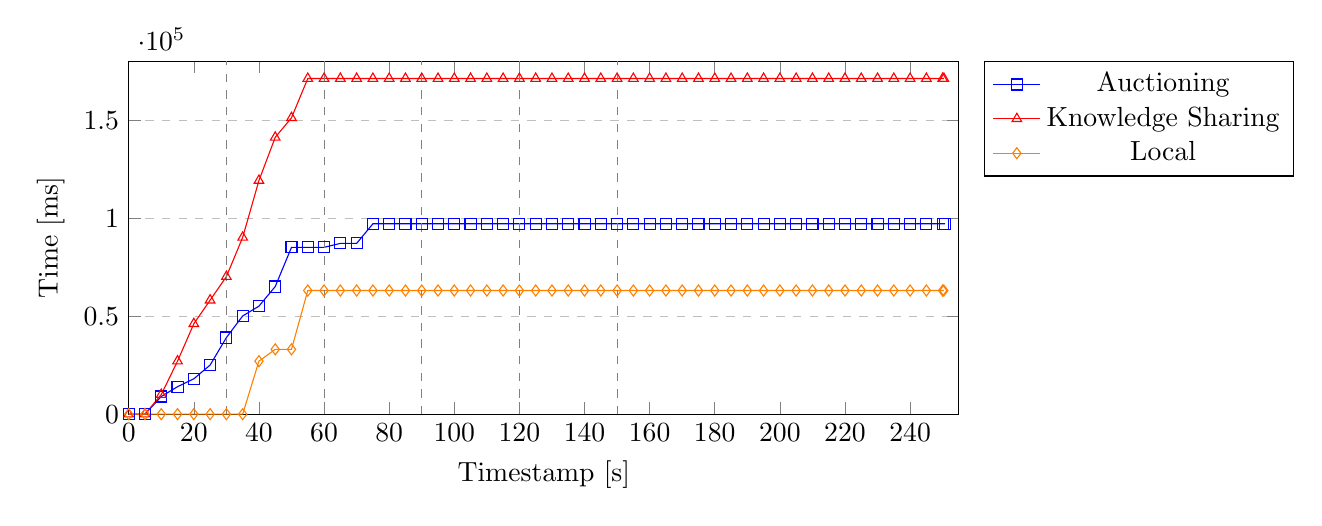
\begin{tikzpicture}
\begin{axis}[
    xlabel={Timestamp [s]},
    ylabel={Time [ms]},
    xmin=0, xmax=255000,
    ymin=0, ymax=180018,
    legend pos=outer north east,
    ymajorgrids=true,
    grid style=dashed,
    width=\textwidth,
    height=0.5\textwidth,
    scaled x ticks=base 10:-3,
    xtick scale label code/.code={}
]

	\addplot[color=blue,mark=square] coordinates {
        (0,0)(5000,0)(10000,9022)(15000,14028)(20000,18038)(25000,25054)(30000,39076)(35000,50106)(40000,55112)(45000,65114)(50000,85122)(55000,85122)(60000,85122)(65000,87124)(70000,87124)(75000,97131)(80000,97131)(85000,97131)(90000,97131)(95000,97131)(100000,97131)(105000,97131)(110000,97131)(115000,97131)(120000,97131)(125000,97131)(130000,97131)(135000,97131)(140000,97131)(145000,97131)(150000,97131)(155000,97131)(160000,97131)(165000,97131)(170000,97131)(175000,97131)(180000,97131)(185000,97131)(190000,97131)(195000,97131)(200000,97131)(205000,97131)(210000,97131)(215000,97131)(220000,97131)(225000,97131)(230000,97131)(235000,97131)(240000,97131)(245000,97131)(250000,97131)(250721,97131)
    };
    \addlegendentry{Auctioning}
	\addplot[color=red,mark=triangle] coordinates {
        (0,0)(5000,0)(10000,10020)(15000,27063)(20000,46118)(25000,58158)(30000,70170)(35000,90181)(40000,119203)(45000,141218)(50000,151223)(55000,171237)(60000,171237)(65000,171237)(70000,171237)(75000,171237)(80000,171237)(85000,171237)(90000,171237)(95000,171237)(100000,171237)(105000,171237)(110000,171237)(115000,171237)(120000,171237)(125000,171237)(130000,171237)(135000,171237)(140000,171237)(145000,171237)(150000,171237)(155000,171237)(160000,171237)(165000,171237)(170000,171237)(175000,171237)(180000,171237)(185000,171237)(190000,171237)(195000,171237)(200000,171237)(205000,171237)(210000,171237)(215000,171237)(220000,171237)(225000,171237)(230000,171237)(235000,171237)(240000,171237)(245000,171237)(250000,171237)(250388,171237)
    };
    \addlegendentry{Knowledge Sharing}
	\addplot[color=orange,mark=diamond] coordinates {
        (0,0)(5000,0)(10000,0)(15000,0)(20000,0)(25000,0)(30000,0)(35000,0)(40000,27063)(45000,33082)(50000,33082)(55000,63089)(60000,63089)(65000,63089)(70000,63089)(75000,63089)(80000,63089)(85000,63089)(90000,63089)(95000,63089)(100000,63089)(105000,63089)(110000,63089)(115000,63089)(120000,63089)(125000,63089)(130000,63089)(135000,63089)(140000,63089)(145000,63089)(150000,63089)(155000,63089)(160000,63089)(165000,63089)(170000,63089)(175000,63089)(180000,63089)(185000,63089)(190000,63089)(195000,63089)(200000,63089)(205000,63089)(210000,63089)(215000,63089)(220000,63089)(225000,63089)(230000,63089)(235000,63089)(240000,63089)(245000,63089)(250000,63089)(250358,63089)
    };
    \addlegendentry{Local}

	\addplot[color=gray, dashed,] coordinates {(30000,0) (30000,180018)};
	\addplot[color=gray, dashed,] coordinates {(60000,0) (60000,180018)};
	\addplot[color=gray, dashed,] coordinates {(90000,0) (90000,180018)};
	\addplot[color=gray, dashed,] coordinates {(120000,0) (120000,180018)};
	\addplot[color=gray, dashed,] coordinates {(150000,0) (150000,180018)};


\end{axis}
\end{tikzpicture}
    \caption{Graph showing the sum of time spent adapting by agents in the growing scenario.}
    \label{fig:adapting-time-growing}
\end{figure}
